\section{Shield LDR}
\subsection{Circuit du Shield LDR}
\begin{figure}[H]
	\centering
	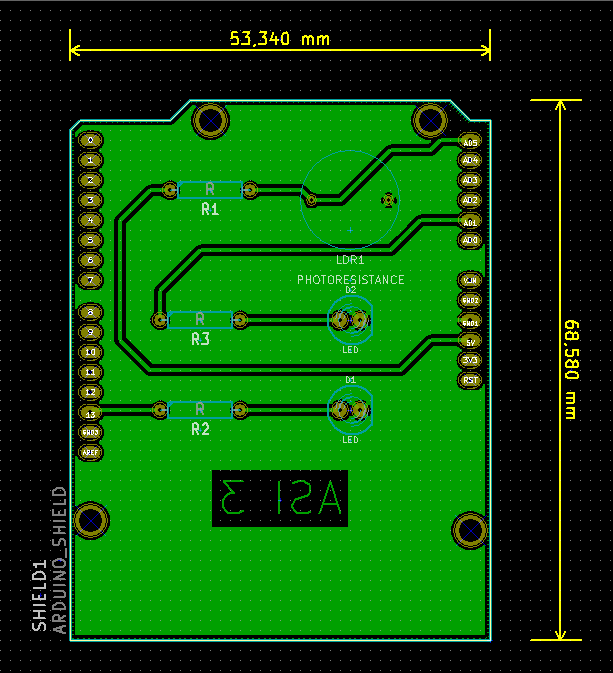
\includegraphics[width=250px]{images/Apercu.png}
	\caption{Logiciel utilisé : Pcbnew de Kicad}
\end{figure}
\newpage
\subsection{Représentation de la carte en 3D}
\begin{figure}[H]
	\centering
	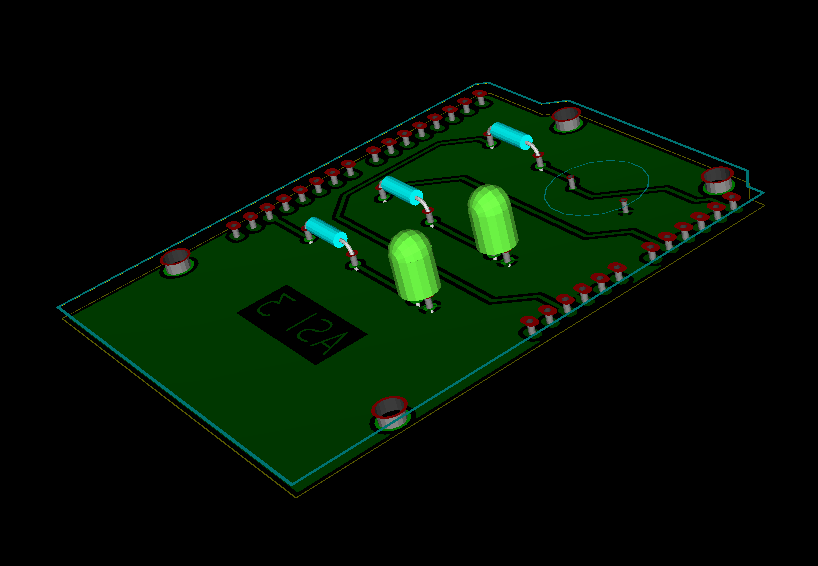
\includegraphics[width=250px]{images/3DLDR.png}
	\caption{Représentation 3D du shield LDR}
\end{figure}
\begin{figure}[H]
	\centering
	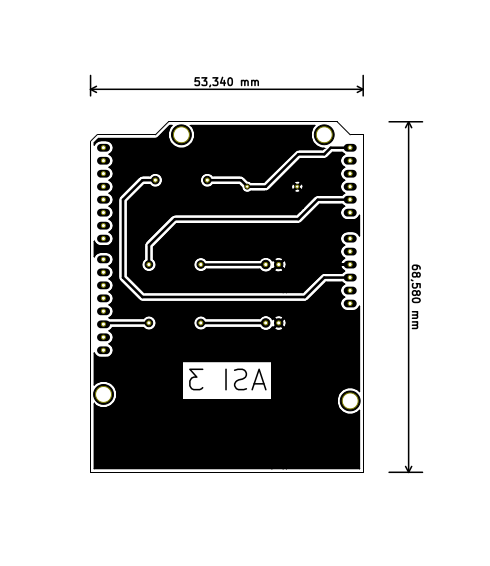
\includegraphics[width=250px]{images/typonLDR.png}
	\caption{Typon du shield LDR}
\end{figure}
%insérer d'autres photos

\subsection{Manoeuvres réalisées sur la carte}
	\subsubsection{Vérification des cartes}
		Test de court-circuit : On a vérifié à l'aide d'un multimètre en mode "test de continuité", si il n'y avait aucunes microcoupures ou court-circuit. Nous en avons recontrés aucun.
	\subsubsection{Assemblage des composants et soudure}
	        Nous n'avons rencontrés aucun problème lors de la soudure et du montage des comoposants.
        

\newpage

\section{Alimentation autonome : 7805}
\subsection{Circuit du régulateur de tension}
\begin{figure}[H]
	\centering
	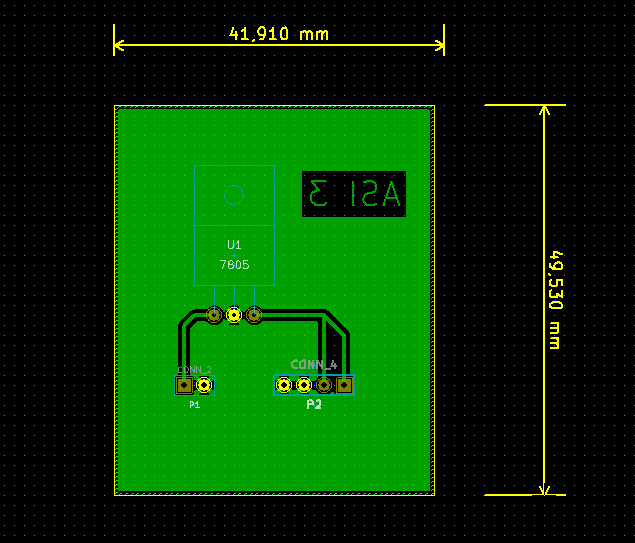
\includegraphics[width=250px]{images/PCB.png}
	\caption{Logiciel utilisé : Pcbnew de Kicad}
\end{figure}

\subsection{Représentation de la carte en 3D}
\begin{figure}[H]
	\centering
	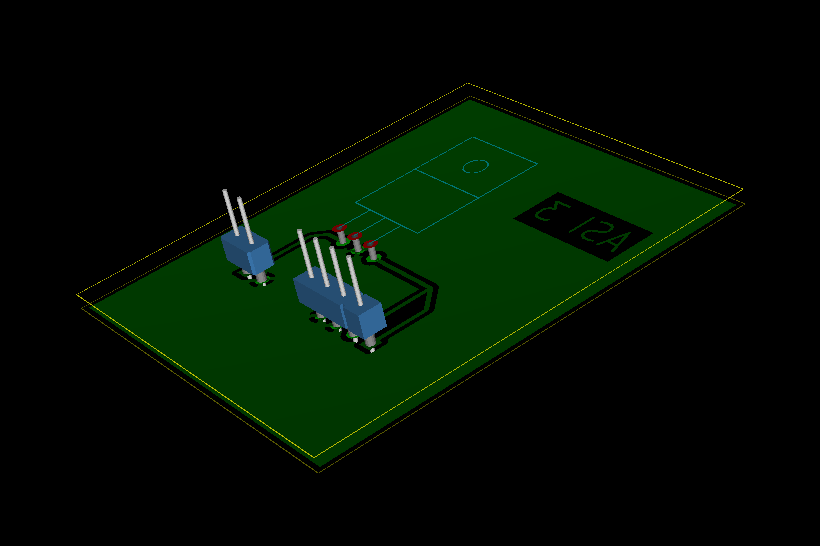
\includegraphics[width=250px]{images/3DReg.png}
	\caption{Représentation 3D de la carte du régulateur}
\end{figure}
\begin{figure}[H]
	\centering
	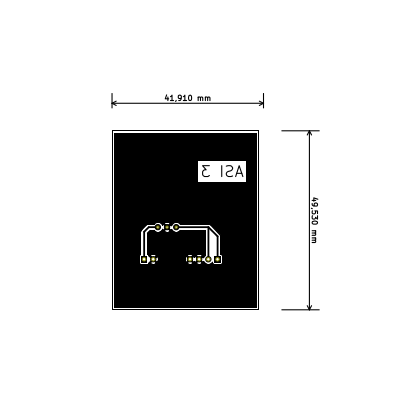
\includegraphics[width=250px]{images/typonReg.png}
	\caption{Typon du régulateur}
\end{figure}
%insérer d'autres photos

\subsection{Manoeuvres réalisées sur la carte}
	\subsubsection{Vérification des cartes}
		Test de court-circuit : On a vérifié à l'aide d'un multimètre en mode "test de continuité", si il n'y avait aucunes microcoupures ou court-circuit. Nous en avons recontrés aucun.
	\subsubsection{Assemblage des composants et soudure}
	%insérer des photos
	Nous avons eu quelques soucis lors de la soudure des composants. En effet deux d'entre nous n'étaient pas habitués à souder. Mais finalement, on eu aucun problème de court circuit. Cependant, dû à la mauvaise qualité du connecteur pour la Raspberry, nous avons des faux contacts qui entraîne la mise sous hors-tension de celle-ci lorsqu'il y a un choc.
